\documentclass[12pt]{article}
\usepackage[table]{xcolor}
\usepackage{graphicx}
\usepackage[hidelinks]{hyperref}
\usepackage{setspace}
\usepackage{pdfpages}
\usepackage[numbers]{natbib}
\usepackage{float}
\usepackage{etoolbox}
\usepackage{longtable}
\apptocmd{\thebibliography}{\raggedright}{}{}
\usepackage{array}
\setlength{\tabcolsep}{18pt}
\renewcommand{\arraystretch}{1.5}
\setlength{\arrayrulewidth}{0.5mm}
\hypersetup{ colorlinks, citecolor=black,
	filecolor=black,
	linkcolor=black,
	urlcolor=blue,
	pdftitle={M.O.S.I.S Proposal Report},
	pdfpagemode=FullScreen,
}
\usepackage{bookmark}
\bookmarksetup{
	numbered,
	open,
}

\usepackage{xcolor}
\begin{document}
\begin{titlepage}
  \begin{center}
    \large{University of Puerto Rico\\
    Mayagüez Campus\\
    \vspace{\baselineskip}
    Department of Electrical and Computer Engineering}
  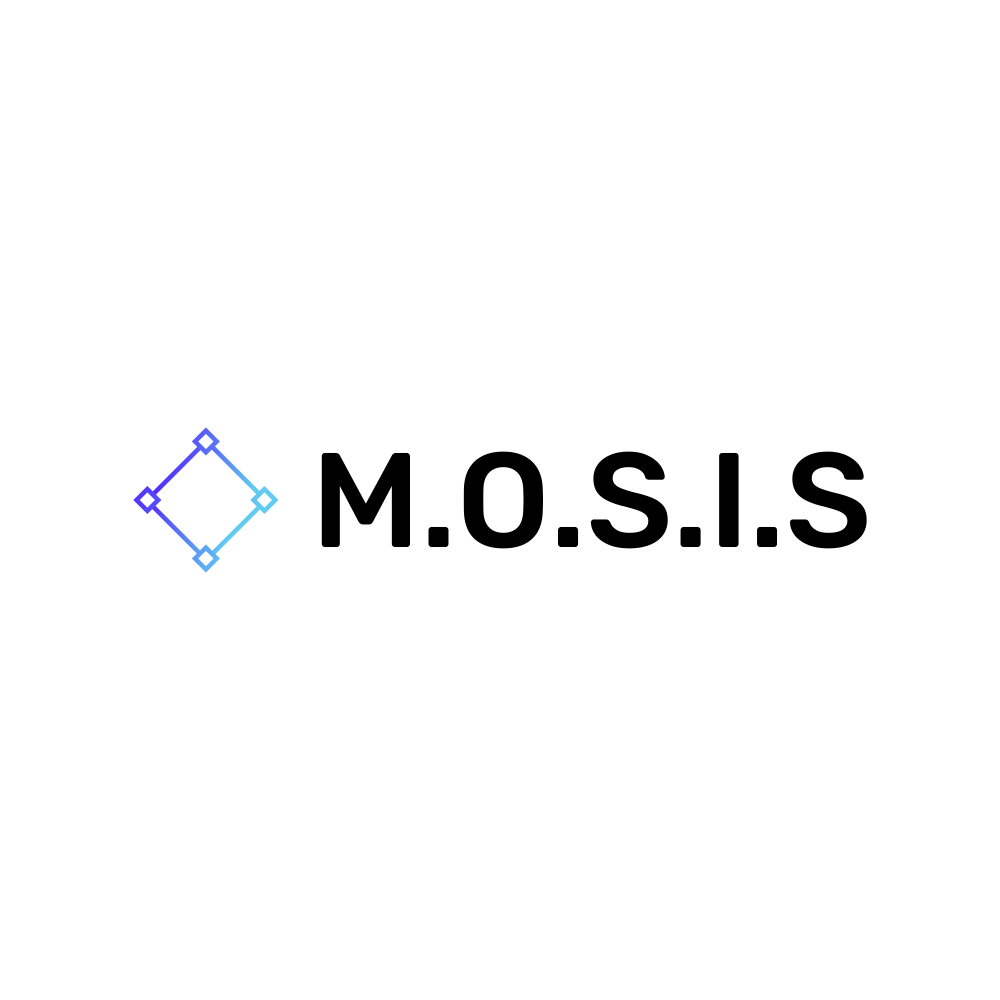
\includegraphics[scale=0.2]{../Title_Page/default.png}\\
    \Huge{\underline{M.O.S.I.S Host Software}\\}
    \Huge{\underline{User Guide}\\}
    \vspace{5cm}
    \large by\\
    Fabio J. Matos Nieves\\
    \normalsize
  \end{center}
\end{titlepage}

\pagenumbering{gobble}
\begin{doublespace}
	 \section*{Executive Summary}
 The existing user interface on the M.O.S.I.S microscope is currently unsuited for the use of the on board buttons and is unwieldy and unreliable for use in the field. This is further compounded by the fact that since the M.O.S.I.S project is aimed at marine researchers and biologists, having such an unpolished user interface is unacceptable. David M. Repollet Otero and Dr. Manuel Jiménez are the major stakeholders in this remake and they are expecting a user interface for the M.O.S.I.S microscope that is easy to use in the field while still providing the basic functionality of the microscope such as capturing media, switching the type of study being performed and the safe shutdown of the system. By the end of the semester it expected that a user interface, database and a standardized folder structure for the captured media be delivered that will comprise a whole product known as M.O.S.I.S U.I  2.0. The key milestones for this project are the front end of the user interface, the database API for the local database, the automated construction of the folder structure from the database and lastly the integration between the front end and back end. The total cost of the project is \$27,802.02 where \$6,172.01 corresponds to the M.O.S.I.S microscope. This microscope can advance \textit{in situ} research and the capabilities for studying marine life. 
\end{doublespace}
\pagenumbering{roman}
\tableofcontents
\newpage
\pagenumbering{arabic}
\begin{doublespace}
	 \section{Problem Statement (Fabio)}
 The Marine Operated Stereoscopic Imaging System (M.O.S.I.S) is an underwater microscope research project developed by Marine Biology Graduate Student David M. Repollet Otero and Dr. Manuel Jiménez.\cite{fernandoguzman3UIMosis2023}\cite{Fabiomatos999} The M.O.S.I.S microscope is used to analyze aquatic habitats \textit{in situ}, since many of the conditions necessary to analyze these environments cannot be replicated in a laboratory setting. The microscope has all of the hardware functions installed and the sensors collect data correctly by one of the two on board microcontrollers.\\ The current M.O.S.I.S microscope has a user interface (U.I) that was developed by a group of various volunteers throughout various semesters. The main issue with the current U.I is that it lacks design cohesion, lacks support for the use of the on board buttons, crashes frequently, and lacks a formal way to store the data captured by the microscope. This is a problem because the microscope will be used underwater by researchers, thus making the current version unusable for that purpose.\\
 The customer for this project is Marine Biologist Graduate Student David M. Repollet Otero. The users will be Graduate student David himself along with other marine biologist researchers working in the field. The stakeholders for this project are Graduate Student David M. Repollet Otero, Dr. Manuel Jiménez, the marine biologist researchers that will be using this U.I along with Fabio J. Matos Nieves and Eduardo S. Miranda Figueroa.\\
 M.O.S.I.S U.I 2.0 proposes to completely re-write the current U.I from scratch in order to ensure a cohesive and tested U.I that can be trusted for \textit{in situ} research. This not only ensures that the research with M.O.S.I.S microscope can be done smoothly but also allows for the media captured by the microscope to be in a standardized format that can even be later analyzed and presented to the researcher automatically.\\
The scope of the project is to re-write the existing M.O.S.I.S microscope U.I from scratch and to redesign the file management systems currently employed by the microscope to be in a standard format.
	\section{Objectives (Eduardo)}
\begin{enumerate}
    \item To design a Graphical User Interface for the M.O.S.I.S project Raspberry Pi capable of capturing media and storing data. 
    \item To deliver a User Interface capable of visualizing the data captured by the M.O.S.I.S project Raspberry Pi.
    \item To create a standardized file system that can be used with any host computer automatically.
    \item To design a local database that can store and backup the data gathered by the M.O.S.I.S project Raspberry Pi.
\end{enumerate}
	\section{Outcomes (Eduardo)}
M.O.S.I.S UI 2.0 will allow the researcher to execute the functions of the microscope with the onboard buttons and can start capturing data with a single button. The onboard screen will present the data captured by the sensors such as temperature, Ph, dissolved oxygen and pressure, and show a live feed of the cameras. In a separate menu the researcher will be able to preview and select a pre-configured study profile of their choosing. After a study is selected the researcher will be able to start/stop the study and shut off the microscope safely. We will be building the new UI with weekly feedback received from the client, adjusting the UI as needed.\\
The new UI will need to connect with the microscope's hardware to gather the necessary data. The adaptation of the existing hardware API will allow the UI to show the live feed footage from the cameras, show updated sensor data and run diagnostics sub-routines at start-up to troubleshoot the hardware. Diagnostics will be executed when the UI starts.\\
The data and metadata gathered by the sensors will then be stored in a standardized format suitable for browsing. The researcher will be able to see the data captured in a file browser. As a added bonus the data captured by the microscope can be analyzed by an external tool. 
	 \section{Methodology and Team Organization (Fabio)}
 The Scrum methodology was chosen because U.I design necessitates constant feedback from the client, which benefits the development cycle in the following ways:\cite{scrumallianceWhatScrum2015}
 \begin{itemize}
 \item Presents a potentially deliverable build of the U.I to the client after each sprint.
 \item The client can give feedback on the build presented to them.
 \item The feedback can either be added to the sprint backlog or incorporated directly into the next sprint deliverable.
 \item The development cycle focuses on presenting deliverables to the client.
 \item Is a lightweight framework of the Agile methodology which allows for self-organization and adaptability.
 \end{itemize}
 To accomplish the project using Scrum we first create a sprint backlog from the objectives signed by the client.\cite{scrumallianceWhatScrum2015} Then a sprint is planned choosing from the sprint backlog, where the Scrum master helps decide what deliverables can be accomplished within a given sprint.\cite{scrumallianceWhatScrum2015}\cite{eyeontechWhatScrumMaster2020} While in the sprint, the Scrum master has daily meeting with the team and asks 3 questions:\cite{eyeontechWhatScrumMaster2020}
 \begin{enumerate}
 \item What did you do yesterday?
 \item What will you today?
 \item What problems impede your progress?
 \end{enumerate}
 The Scrum master then helps the team reach consensus, keeps the team focuses and removes any obstacles impeding progress.\cite{eyeontechWhatScrumMaster2020}\\
 For testing and quality assurance for the U.I, we will be meeting with the client on a weekly basis to assure that the U.I meets their standards and have the client test the U.I in meeting. To supplement this, during development, pair programming will be employed in order to reduce bugs and to test software by a different person that is not the developer. For the back-end elements, unit and integration tests will be extensively used to ensure that the expected output is correct, for both single modules and the interface between modules. This strategy reduces the time for successful module integration.\\
 The work will be broken down as follows:
 \begin{enumerate}
 \item The client creates a sprint backlog.
 \item A sprint is planned with the Scrum master helping in deciding if the tasks within the sprint are feasible.
 \item At the beginning of the day during the sprint, a stand up meeting is held with the team and the Scrum master focuses the team along with mediating and resolving problems that impede progress.
 \item A potentially deliverable build of the U.I (alpha or beta) is shown to the client during the weekly meeting.
 \item The client gives feedback on the build shown to them.
 \item The feedback is incorporated into either a new sprint item or address into the next sprint.
 \item Repeat steps 2-6 until all items from the sprint backlog have been completed.
 \end{enumerate}
 For team organization, Fabio J. Matos Nieves will be both Scrum master,project manager and lead font-end developer while Eduardo S. Miranda Figueroa will be the lead back-end developer.
	
 \section{Budget (Eduardo)}
 The budget for the M.O.S.I.S project is divided into 3 major categories, those being Human Resources, Equipment and Facility. Human Resources includes the labor costs of a average entry level software engineer in Puerto Rico\cite{SoftwareEngineerSalary}. Equipment are those costs that include the software programs and hardware components required for the development of the project. The facility costs are related to the location in where the development of the project will occur. The following table includes the summary of costs:
 \begin{table}[H]
    \centering
    \begin{tabular}{||c | c||} 
     \hline
     \rowcolor{cyan}
     Category & Cost \\ [0.5ex] 
     \hline
     Human Resources & \$18,430.61\\ 
     \hline
     Equipment & \$7,961.98\\
     \hline
     Facility & \$1,410.00\\
     \hline
     \rowcolor{teal}
     Total Estimated Cost & \$27,802.02\\
     \hline
    \end{tabular}
    \caption {Total Estimated Cost of the Project}
    \label {table:1}
\end{table}
The Overhead costs of the project are:\\
\textit{\$27,802.02 * 1.5 = \$41,703.03.}
%\\The Overhead for this project is calculated by:
%\begin{figure}[h]
%  $$\frac{\textit{Indirect Costs}}{\textit{Direct Costs}} * 100 = \frac{3,538.61}{24,263.98} * 100 = 14.58\%$$
%\caption{The Overhead cost of the Project}
%end{figure} 
\\\textbf{Appendix C} contains more detailed explanation of the budget for the project.
	 \section{Project Schedule (Fabio \& Eduardo)}

\end{doublespace}
 \bibliographystyle{IEEEtranN}
 \bibliography{../../Refeferences Library/ICOM5047.bib}

\newpage
\appendix
\section{Resumes}
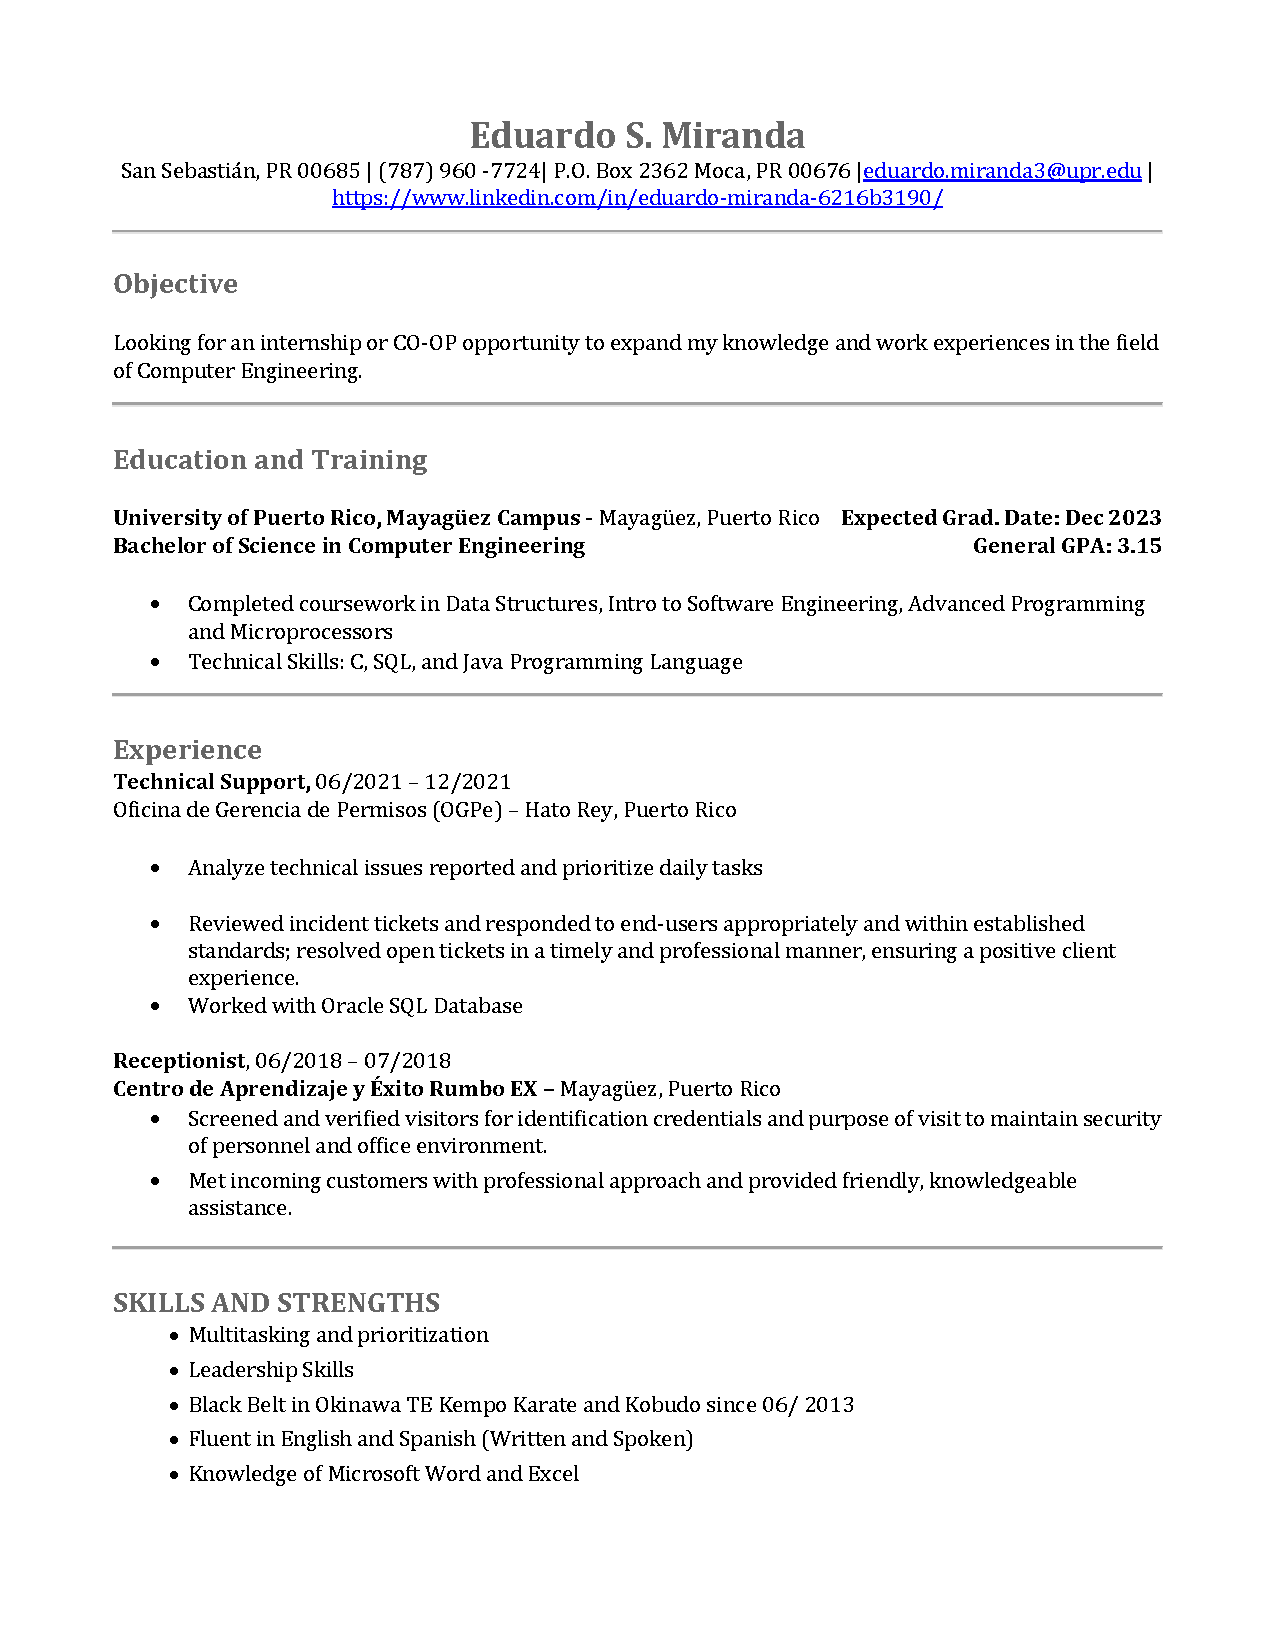
\includepdf[pages=-]{./Appendices/Resumes/Figures/Resume - Eduardo Miranda.pdf}
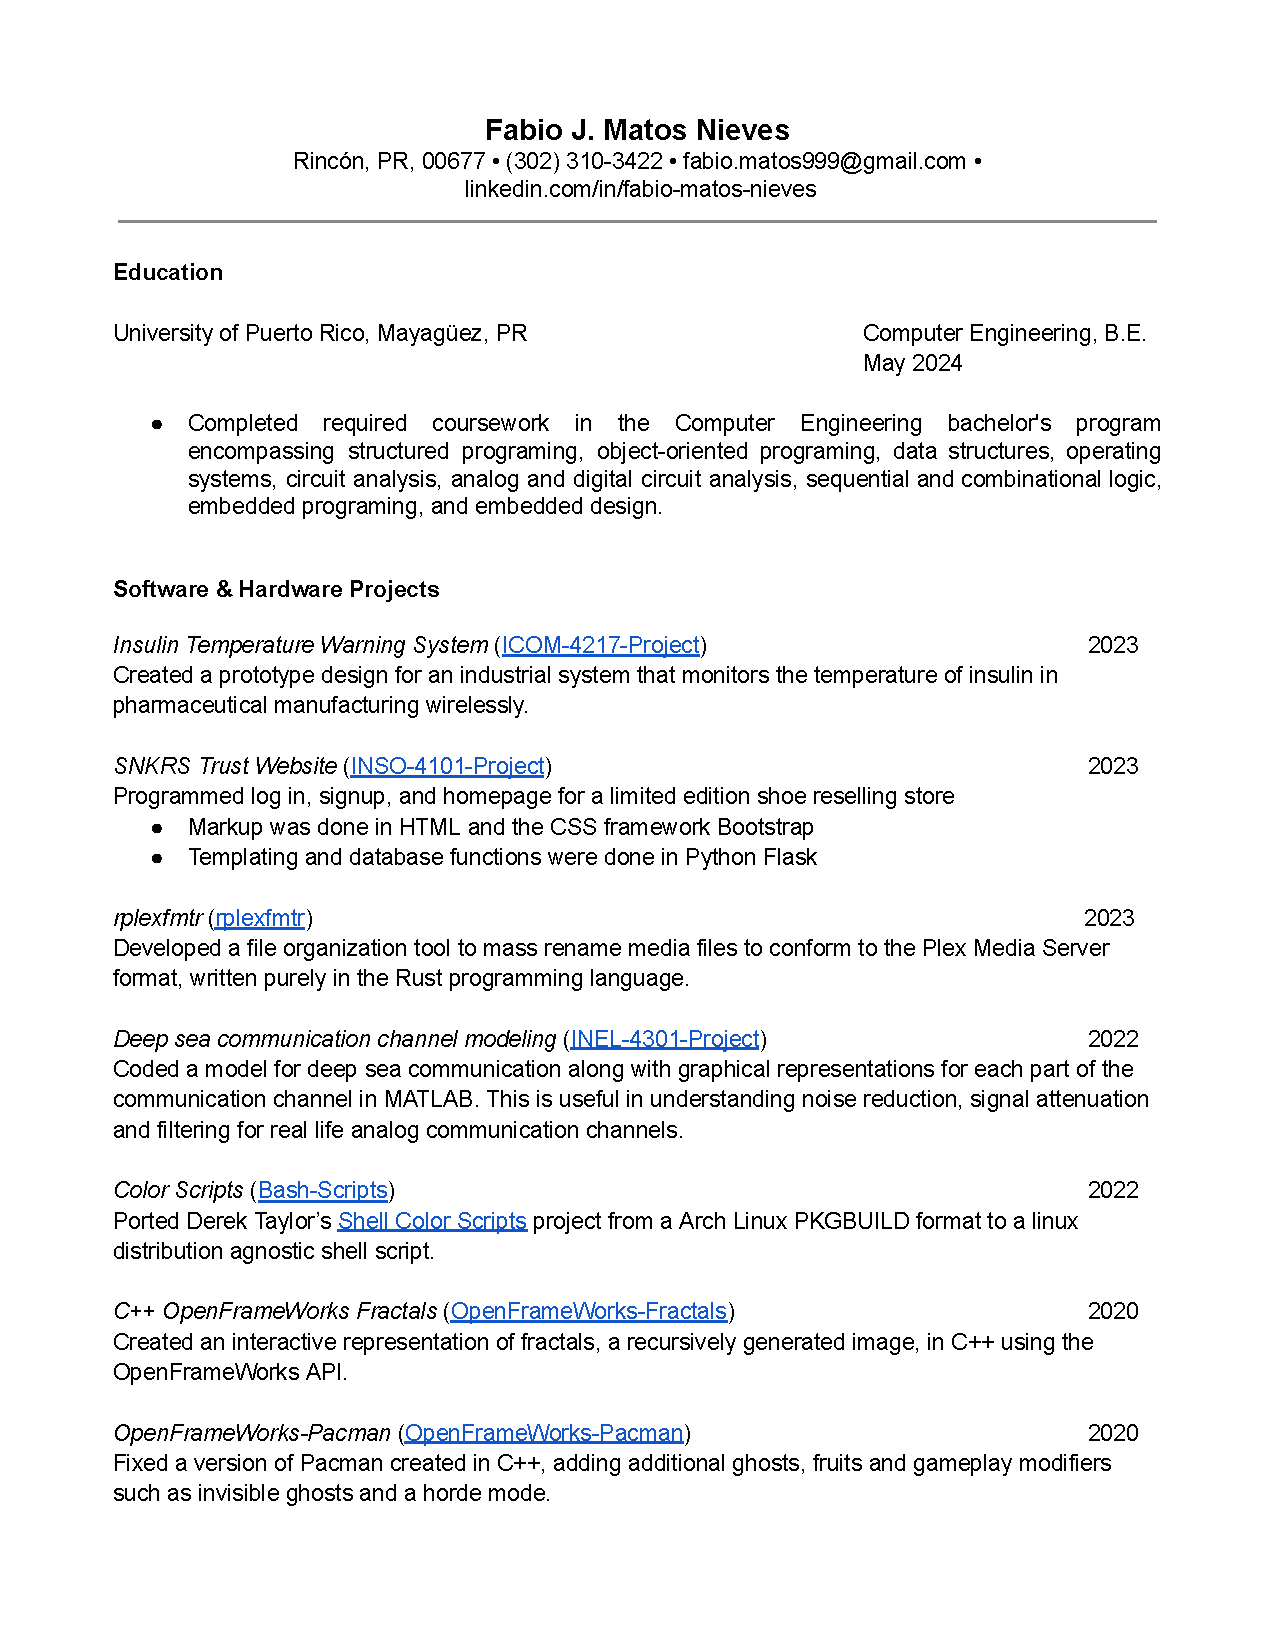
\includepdf[pages=-]{./Appendices/Resumes/Figures/Fabio J. Matos Nieves Resume 2023.pdf}
 \section{Progress Assessment \& Metrics}

 \section{Detailed Budget Calculations \& Justifications (Eduardo)}
 Human Resources includes labor costs of each member.  Each salary is detailed with hours per week and working weeks during the project.\\
 \begin{table}[H]
    \centering
    \textbf{Human Resources}
    \begin{tabular}{||m{0.15\textwidth}|m{0.15\textwidth}|m{0.1\textwidth}|m{0.1\textwidth}|m{0.1\textwidth}|m{0.1\textwidth}||}
     \hline 
     \rowcolor{cyan}
     Name & Role & Stipend & Work Hours /Week & Working Weeks & Salary\\
     \hline
     Fabio J. Matos Nieves & Software Engineer /Project Manager& \$20.90 & 30 & 13 & \$ 8,151.00\\ 
     \hline
     Eduardo S. Miranda Figueroa & Software Engineer & \$20.90 & 30 & 13 & \$ 8,151.00\\
    
     \hline 
     \rowcolor{teal}
     \multicolumn{3}{||c|}{Total Cost} & \multicolumn{3}{c||}{\$16,302.00}\\
     \hline
    \end{tabular}
    \caption {Human Resources Wages}
    \label{table:2}
\end{table}
Fringe Benefits are bonus benefits that are given by the employer and applies to each employee.\\
\begin{table}[H]
    \centering
    \textbf{Fringe Benefits\cite{WhatAreFringe}}
    \begin{tabular}{||m{0.225\textwidth}|m{0.225\textwidth}|m{0.2\textwidth}|m{0.2\textwidth}||}
        \hline 
        \rowcolor{cyan}
        Fringe Benefits & Cost per Employee & Quantity & Cost\\
        \hline
        Social Security &  \$ 623.55 & 2 & \$ 1,247.10\\ 
        \hline
        Health Insurance & \$400 & 2 & \$ 800.00 \\
        \hline
        401K & \$ 40.76 & 2 & \$ 81.51\\ 
        \hline 
        \rowcolor{teal}
        \multicolumn{2}{||c|}{Total Cost} & \multicolumn{2}{c||}{\$2,128.61}\\
        \hline
       \end{tabular}
       \caption {Fringe Benefits Costs}
       \label{table:3}
       $\textnormal{Social Security} = \%7.65 * Salary$\\
      \textit{Formula 1: Social Security Calculations}\\
        $\textnormal{401k} = \%5 * Salary$\\
        \textit{Formula 2: 401k Calculations}
       
\end{table}
Equipment costs are those of the hardware and software that will be used during the project. For this project the programming will be done with 2 laptops and a course of udemy will help us with coding.\\
\begin{table}[H]
    \centering
   \textbf{Equipment Costs}
    \begin{tabular}{||m{0.275\textwidth}|m{0.225\textwidth}|m{0.110\textwidth}|m{0.15\textwidth}||}
        \hline 
        \rowcolor{cyan}
        Item & Price & Quantity & Cost\\
        \hline
        Acer Nitro 5 Laptop & \$739.99 & 1 & \$739.99\\
        \hline
        LG Laptop Gram&  \$1020.00 & 1 & \$1,020.00\\ 
        \hline
        Udemy "Python GUI Development with PyQt6 \& Qt Designer" Class & \$14.99 & 2 & \$ 29.98 \\
        \hline
        M.O.S.I.S Microscope & \$6,172.01 & 1 & \$6,172.01\\
        \hline
        \rowcolor{teal}
        \multicolumn{2}{||c|}{Total Cost} & \multicolumn{2}{c||}{\$7,961.98}\\
        \hline
       \end{tabular}
       \caption {Equipment Costs}
       \label{table:4}
\end{table}
Facility Costs are those of the work area where both members will develop the M.O.S.I.S project. The following costs are an approximation of the services provided. \\
\begin{table}[H]
    \centering
    \textbf{Facility Costs}
    \begin{tabular}{||m{0.225\textwidth}|m{0.225\textwidth}|m{0.2\textwidth}|m{0.2\textwidth}||}
        \hline 
        \rowcolor{cyan}
        Item & Price & Quantity & Cost\\
        \hline
        Rent &  \$ 350.00 per month & 3 & \$1,050.00\\ 
        \hline
        Power & \$45.00 per month & 3 & \$135.00 \\
        \hline
        Water & \$ 25.00 per month & 3 & \$75.00\\ 
        \hline
        Internet& \$ 50.00 per month & 3 & \$150.00\\ 
        \hline
        \rowcolor{teal}
        \multicolumn{2}{||c|}{Total Cost} & \multicolumn{2}{c||}{\$1,410.00}\\
        \hline
       \end{tabular}
       \caption {Facility Costs}
       \label{table:5}
\end{table}
\begin{table}[H]
    \centering
    \textbf{Total Estimated Cost}
    \begin{tabular}{||m{0.125\textwidth}|m{0.133\textwidth}|m{0.125\textwidth}|m{0.125\textwidth}|m{0.225\textwidth}||}
        \hline 
        \rowcolor{cyan}
        Category & Human Resources & Equipment & Facility & Total Estimated Cost\\
        \hline
        \rowcolor{teal}
        Cost & \$18,430.61 & \$7,961.98 & \$1,410.00 & \$27,802.02\\
        \hline
    \end{tabular}
    \caption {Total Estimated Cost of The Project}
       \label{table:6}
\end{table}
The Overhead costs of the project are:\\
\textit{\$27,802.02 * 0.5 = \$13,901.01.}\\
The total cost of the project with the Overhead is:\\
\textit{\$41,703.03}
\section{Risk Management (Fabio)}
\rowcolors{2}{black!20}{black!10}
\begin{longtable}{|m{0.2\textwidth}|m{0.2\textwidth}|m{0.5\textwidth}|}
	\hline
	\textbf{Risk}                                                  & \textbf{Likelihood} & \textbf{Contingency Measures}                                                                                                                                            \\ \hline
	One or more of the camera feeds fail                           & Medium              & Add diagnostic information to startup and log error to console and log file.                                                                                             \\ \hline
	The Tiva microcontroller UART fails                            & Low                 & Prevent U.I startup if failure is detected and log error to console and log file.                                                                                        \\ \hline
	The microscope casing is leaking                               & High                & Detect the leak using the onboard sensor, log to a log file and initiate a graceful shutdown.                                                                            \\ \hline
	The database becomes corrupted.                                & Low                 & Reconstruct database from folder structure.                                                                                                                              \\ \hline
	The screen malfunctions                                        & Low                 & Unrecoverable                                                                                                                                                            \\ \hline
	The on board buttons fail                                      & Medium              & In the field it is unrecoverable but can be operated via a wireless mouse on land.                                                                                       \\ \hline
	The RTOS becomes corrupted                                     & Low                 & The data is stored in a waterproof and shockproof solid state disk, thus the data is unaffected and the microscope will be periodically backed up via the Host Software. \\ \hline
	There is a worker strike on campus                             & High                & Complete hardware API at an expedited pace                                                                                                                               \\ \hline
	There is a hurricane that immobilizes action in the university & High                & Unrecoverable                                                                                                                                                            \\ \hline
	One of the team members becomes ill or drops the course        & Low                 & Discuss with the client workload adjustment measures                                                                                                                     \\ \hline
	\caption{Risk Table}
	\label{tab:RiskTable}
\end{longtable}

\section{Market Overview (Fabio)}
Since this is a purpose built user interface for a embedded system research project, there is no potential market for this project. There is one research project for underwater microscopy from Andrew D. et. all.\cite{mullenUnderwaterMicroscopySitu2016} But the potential market for the M.O.S.I.S microscope and its accompanying software could be modestly big. It would mainly be used as a research device for universities, thus the total market size would be small. However, since it is a complete research tool for marine researchers, it could potentially be popular within that specific segment of the population.
 \section{Gantt Chart and Project Management Tools (Fabio \& Eduardo)}
 The Gantt Chart is in the following page:
 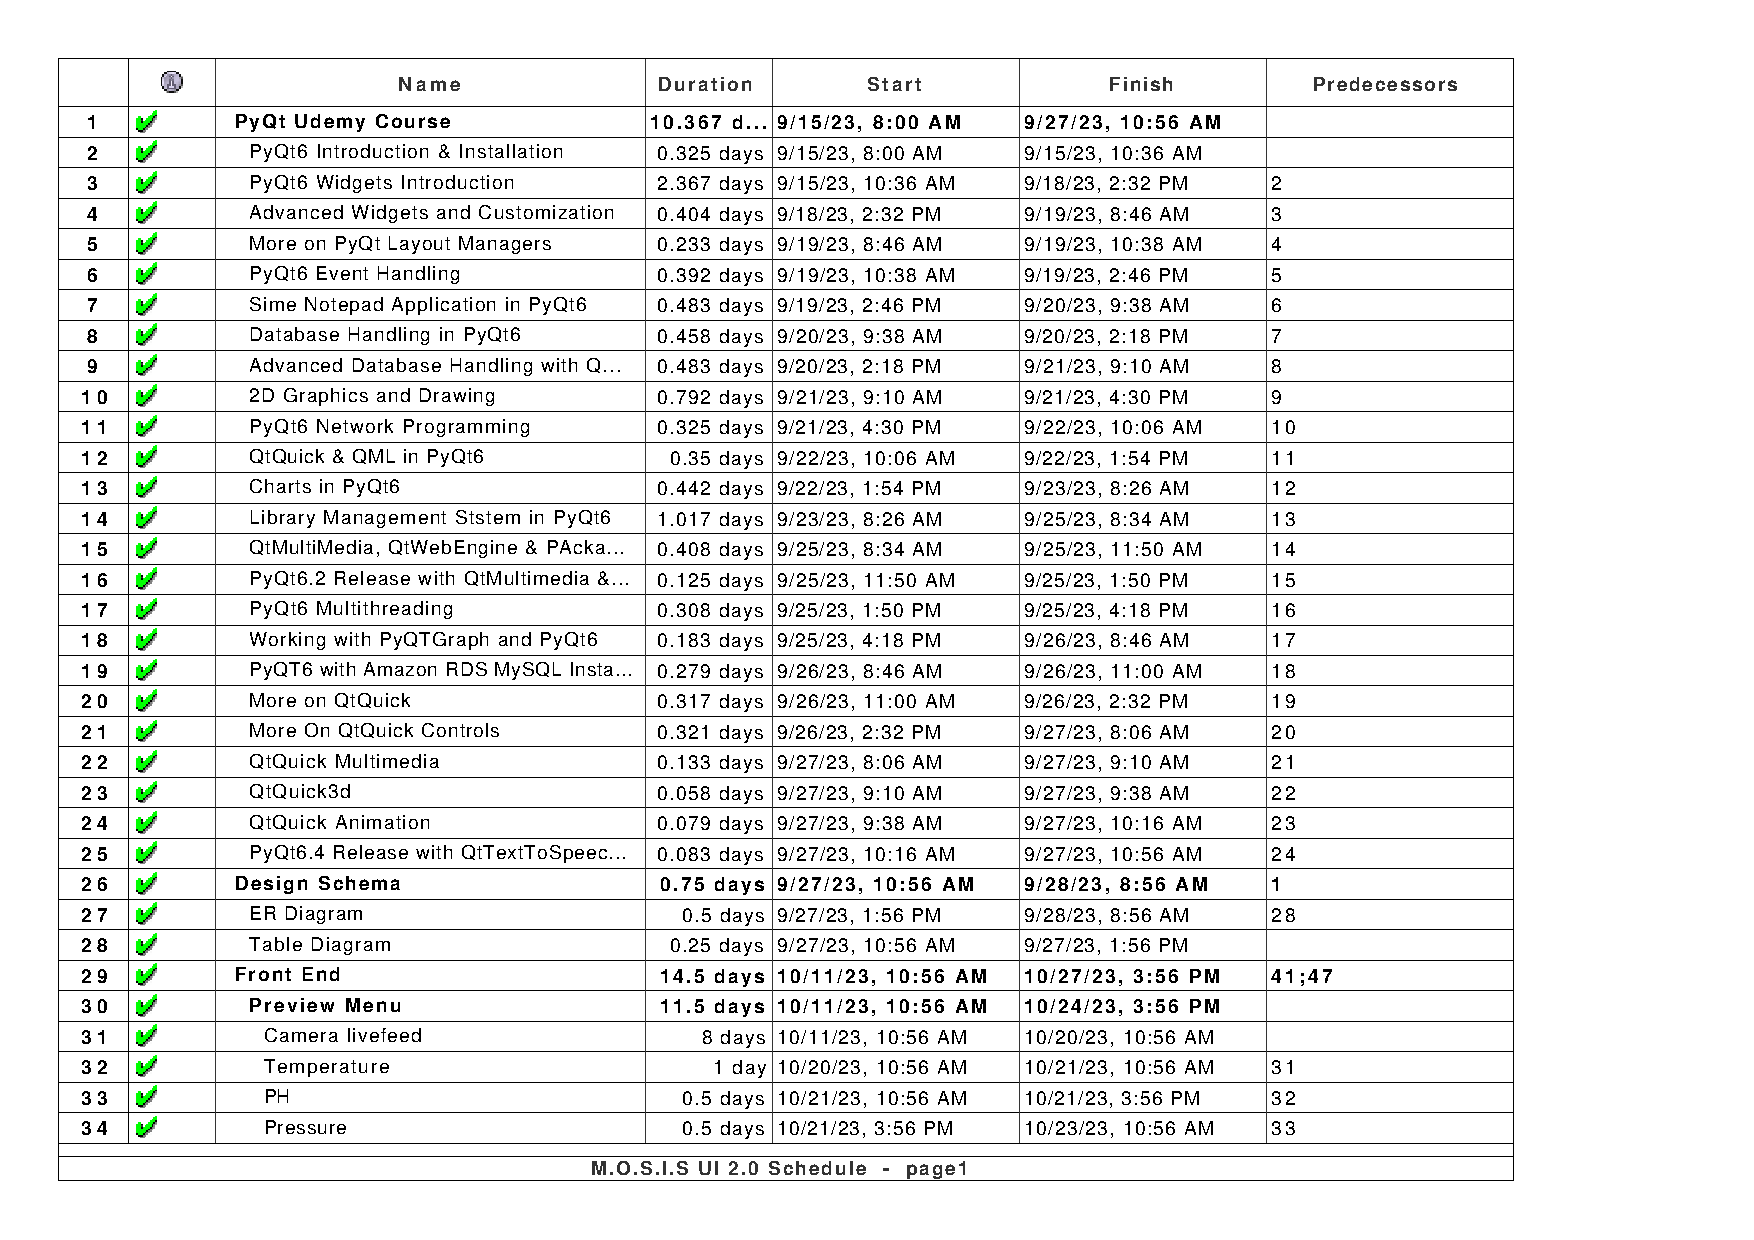
\includepdf[pages=-]{./Project Schedule/M.O.S.I.S UI 2.0 Schedule.pdf}
\section{Client's Signature with Objectives}
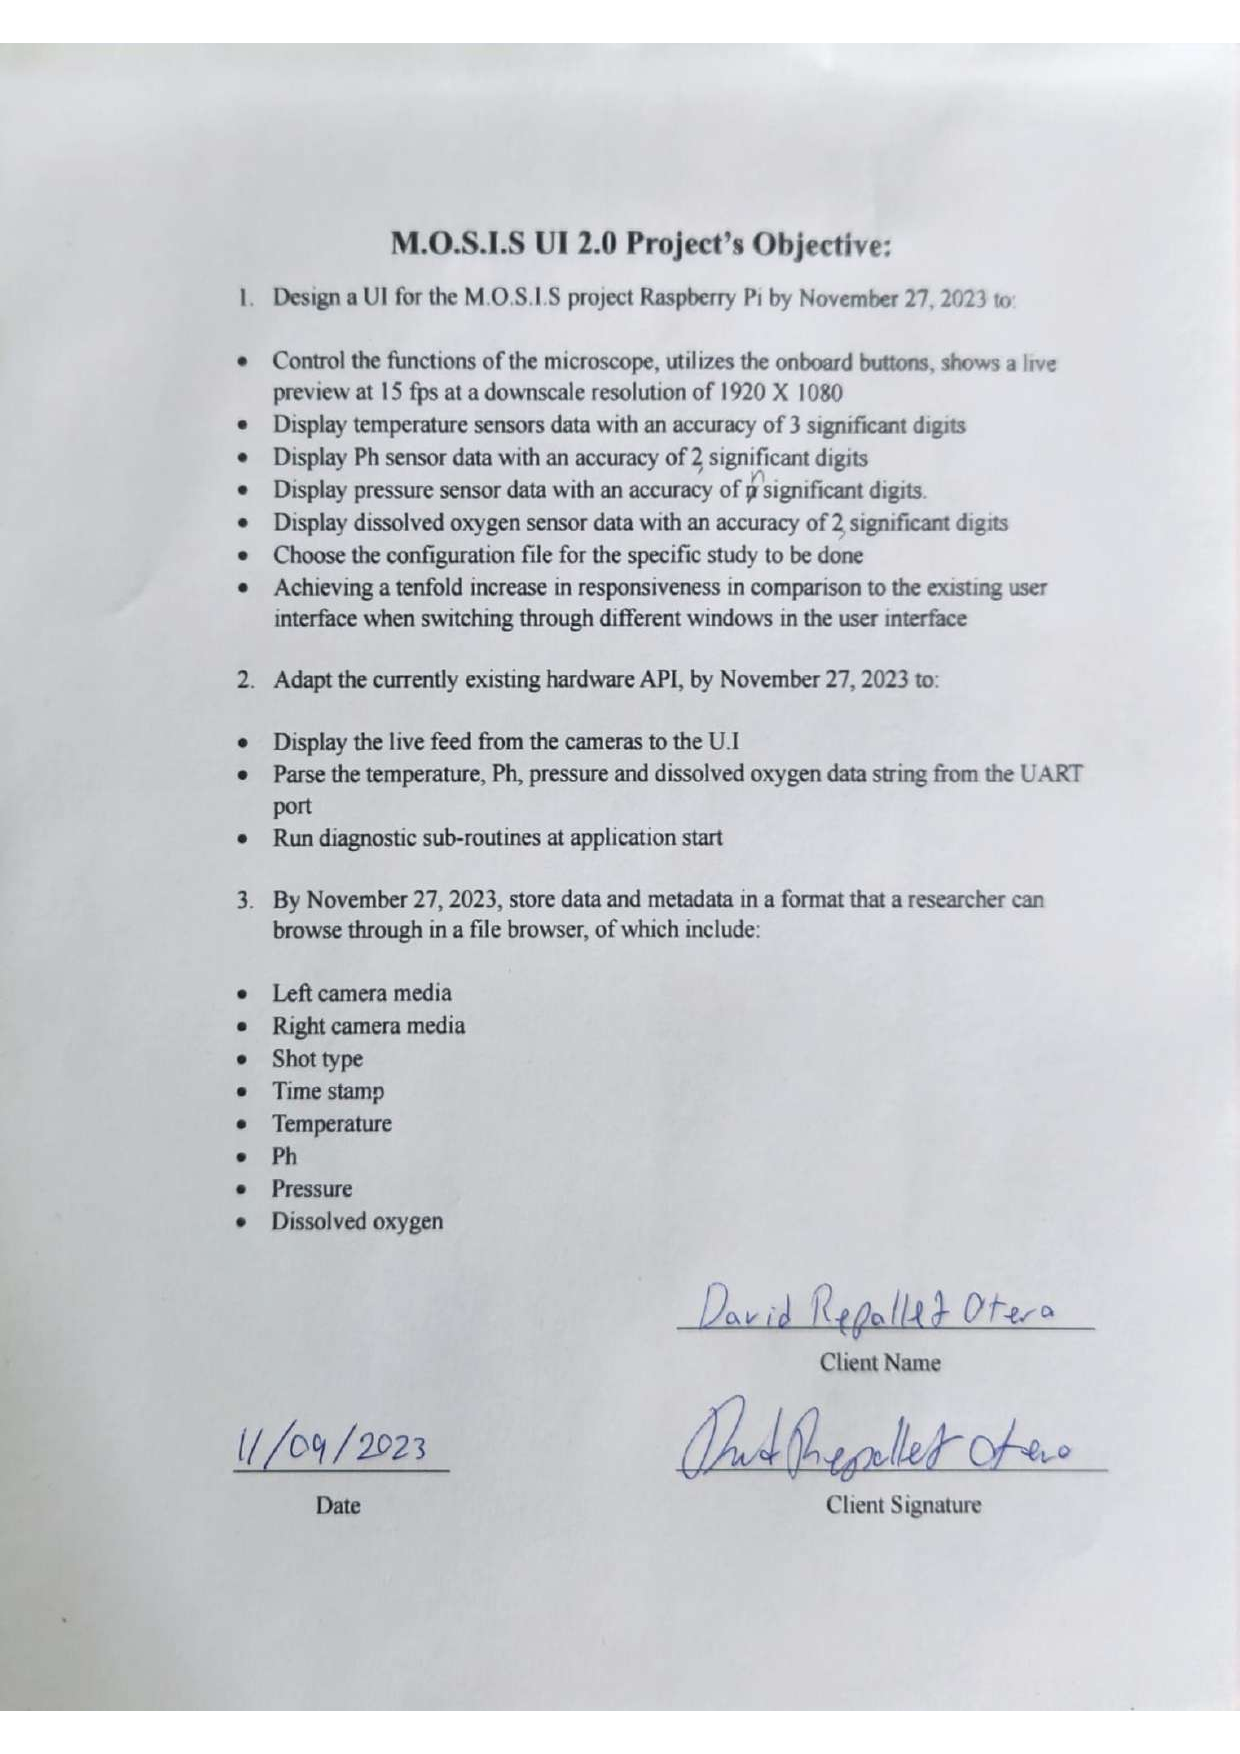
\includepdf[pages=-]{./Appendices/Client's Signature with Objectives/Figures/ClientSignature.pdf}
\end{document}